\documentclass[12pt,a4paper]{article}

\usepackage{graphicx}
\usepackage{fancyhdr}
\usepackage{color}
\usepackage[hidelinks]{hyperref}

\renewcommand\thesection{\arabic{section}}

\title{
\includegraphics[scale=0.5]{Graphics/BASU_Logo_header.png}\\[20pt] {\Huge \emph{Final FOP Project}}}
\author{Matin Amirpanah far\thanks{email: matin.a0789@gmail.com}\\
	\texttt{student NO:40212358003}\and
	Nima Makhmali\thanks{email: nmkhmly790@gmail.com}\\ \texttt{student NO:40212358035}}
\date{\today}

\fancyhf{}
\fancyhead[L]{Final FCP Project}
\fancyhead[R]{Bu-Ali Sina Univercity}
\fancyfoot[C]{\thepage}
\pagestyle{fancy}



\begin{document}
	
	\maketitle
	
	\newpage
	\tableofcontents
	
	\newpage
	\setcounter{section}{0}
	\part{Introducing the game}\label{introducing}
        	
	\section{How to Play}\label{introducing.how}
	  This game which we have typed the code, when we start it, it prints a menu on the page for the user, and by clicking the start of the program, it asks the user to enter a number for the number of rows and columns of the game page, and then the game page is printed, which is a The ship is on the last line of this page
	\section{Errors and Warnings}\label{introducing.errors}
	
	
	\newpage
	\setcounter{section}{0}
	\part{Code description}\label{description}
	
	\section{libraries}\label{description.libraries}
	We have used the following libraries in this code
	\subsection{iostream}
	This library is a requirement for writing any c++ code.
	\subsection{stdlib.h}
	We used this library so that we can use "rand()" and "srand()" functions.
	\subsection{ctime}
	By adding this library, we were able to use the "sleep()" function for interrupts.
	\subsection{fstream}
	Adding this library is so that we can create a file and use its commands like "fstream" or "ios::binary".
	\subsection{vector}
	We used this library to be able to use vector and its functions in the code, such as "push\_back".
	\section{Defines}\label{description.defines}
	In this code, we have used defines for colors such as blue, green, black, etc., to color and also to bold our output text, whose ascii codes we have obtained by searching the internet, 
	which of course We also used it in the mini project and we have also put 4 defines for the keys of our game in the code.
	\section{Structures}\label{description.structs}
	We have used an enum and three structures in this code
	\section{Functions}\label{description.func}
	Our code functions are as follows
	\subsection{main}
	This function is actually our main function, and first it calls the menu function, then it checks the condition of the heal of the ship, whether the heal of the spaceship is more than 0 or not.
    Another task of this function is to print the checkerboard of the game, which calls the grandDraw function
    Then it does the work of moving the enemies and the spaceship and saving the game information.
	
	\subsection{grandDraw}
	This function has the task of printing the game page, if we select newGame in the menu, it first takes a number from the user and prints the number of rows and columns equal to that number.
    At the top of the game page, we have the name of the game, Final Fight, and the heal ship, in this function, we call the horizontalLineDraw function to print the lines.\\ \\
	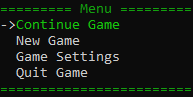
\includegraphics[scale = 1]{Graphics/menu.png}
	\subsection{horizontalLineDraw}
	This function has the task of printing the horizontal lines of the game map by using two for loops
	\subsection{menu}
	Our menu function, what it displays, consists of four sections, which we first use a do while loop to display once, and then according to the definitions at the top of the code using the ascii code, the up and down buttons and left
	and we have defined correctly, we can choose the options, by selecting any of the options, we will enter the switch and case section of this function, each of which applies commands.\\ \\
	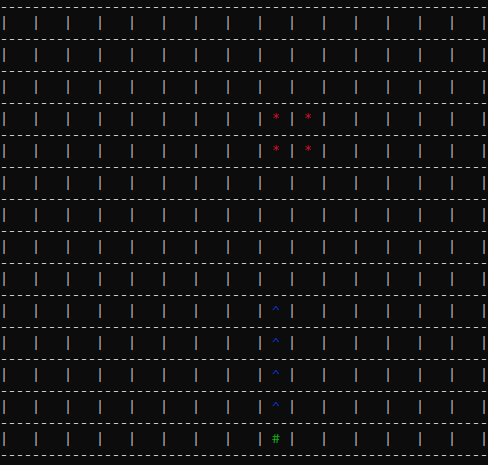
\includegraphics[scale = 1]{Graphics/map.png}
	\subsection{newGame}
	If the user selects the second option i.e. newgame in the game menu, 
	this function will be called and at first it will ask the user for the number of rows and columns of the game screen and after waiting for the user to enter the target point after entering these two numbers of the game screen will be printed.
	\subsection{gameSetting}
	If the user selects the second option in the game menu, i.e. game setting, this function will be called. When it is selected, 
	three options will be printed on the screen, which include changing the character of the ship and the enemy and returning to the menu. If we choose any of the two options to change the character, 
	the system will ask us for the new character and then change it.
	\subsection{move}
	Using a do while loop, this function first receives commands from the user once, then by using switch case and the right, left, down and up keys,
	whose codes have been defined as define at the top of the program, the commands are sent to the ship. If we select the right or left key,
	according to the program code, the current position of the ship will be empty and its line will be moved by one unit, and if we select the down key,
	the shoot function will be called.
	\subsection{shoot}
	In the shoot function, we create a new variable called newbullet using the bullet structure, 
	and position the ship's beam according to the two variables x and y that we introduced in the structure.
	 %Finally, we use the push_back function, which is in the vector class.
	\subsection{save}
	We have used the fstream library to use this function.
    In this function, we first create a file, of course, the information in this file is stored in binary form because we have used the structure, and to transfer information from the structure to the file, this command must be used (ios::binary).
    Then we have used the flush command, which puts the information in the file part by part
	\subsection{load}
    The structure of this function is the same as the save function. This function reads the saved information of the game, of course, this is a binary operation with the same file "saveFile.bin".
    When we select continue game option in the menu, since the information was saved in the file in a piece by piece, from where the game left off.
    He starts to continue
    If the user has exited the game, the file is also deleted, so there is no information to display.
    This discussion, which was said to continue the game after reading the file, continues the game with those for loops and the new command.
	\newpage
	\setcounter{section}{0}
	\part{links and references}\label{linkAndRef}
	
	\section{Links}\label{linkAndRef.links}
	\subsection*{project's GitHub link}
	\href{https://github.com/Matin0789/FinalFight.git}{\color{blue}{https://github.com/Matin0789/FinalFight.git}}\\
	\subsection*{Ask question on StackOverflow}
	\href{https://stackoverflow.com/questions/78055082/crashing-a-c-codes}{\color{blue}{https://stackoverflow.com/questions/78055082/crashing-a-c-codes}}\\
	
	\section{References}\label{linkAndRef.ref}
	\href{https://www.geeksforgeeks.org/c-plus-plus/}{\color{blue}{https://www.geeksforgeeks.org/c-plus-plus/}}\\
	\href{https://www.programiz.com/cpp-programming}{\color{blue}{https://www.programiz.com/cpp-programming}}

	 

\end{document}
